\chapter{The Australian Scenario}\label{Australiano}

Figure \ref{fig:lrmujeres} shows the percentage of women aged 14--26 infected after starting the vaccination program in both simulated scenarios. The fast decrease in both scenarios can be seen at the very~beginning.
\vspace{-24pt}

\begin{figure}[H]
	\centering
	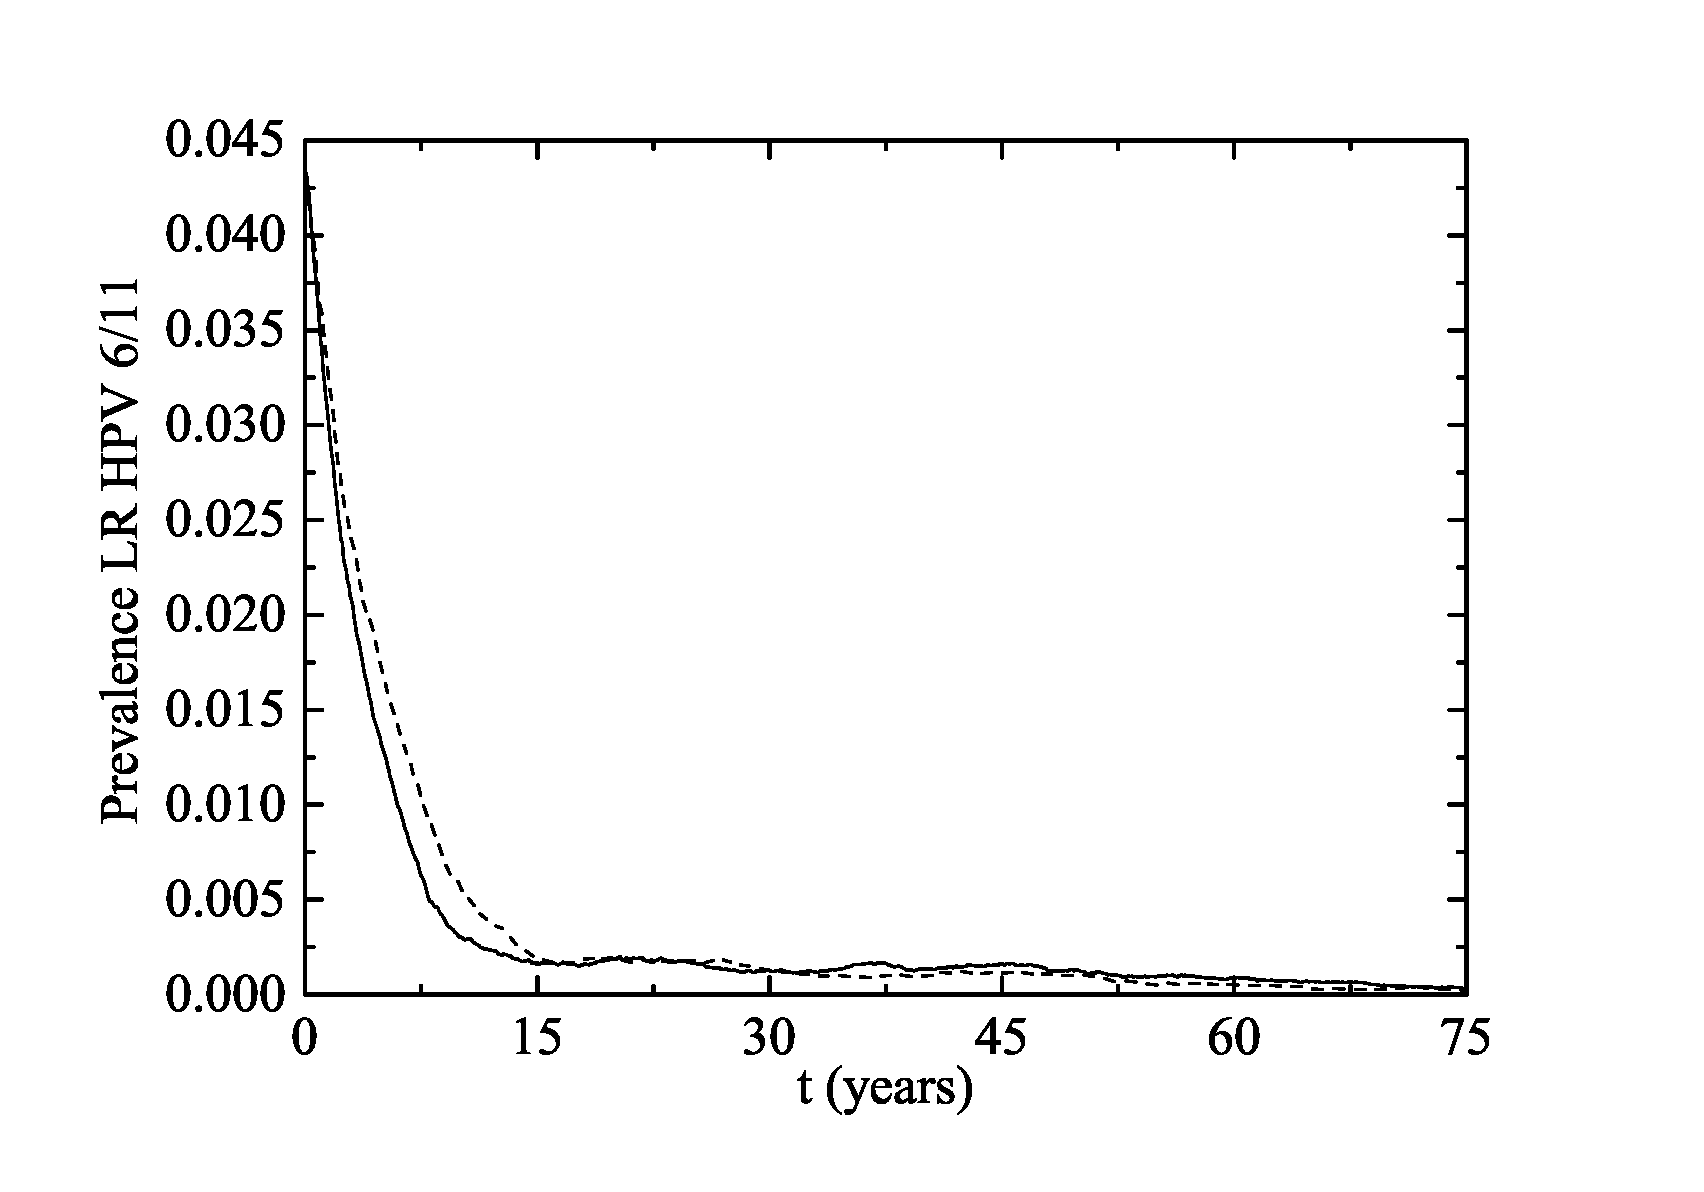
\includegraphics[scale=0.4]{FigLRwomen.pdf}
	\vspace{-12pt}
	\caption{Percentage of women aged 14--26 infected of LR HPV 6 and/or 11 after the 
%Pls define
%ANSWER: we did not find anything highlighted	
implementation of the vaccination program (Scenario 1: solid line and Scenario 2: dotted line).}
	\label{fig:lrmujeres}
\end{figure}

In Figure \ref{fig2}, we have plotted the same data as in Figure \ref{fig:lrmujeres} but from another point of view: the~average percentage of decline of women infected of LR HPV 6 and/or 11. As the vaccination program progresses over time, the percentage of decline obviously grows. 
\vspace{-24pt}
\begin{figure}[H]
	\centering
	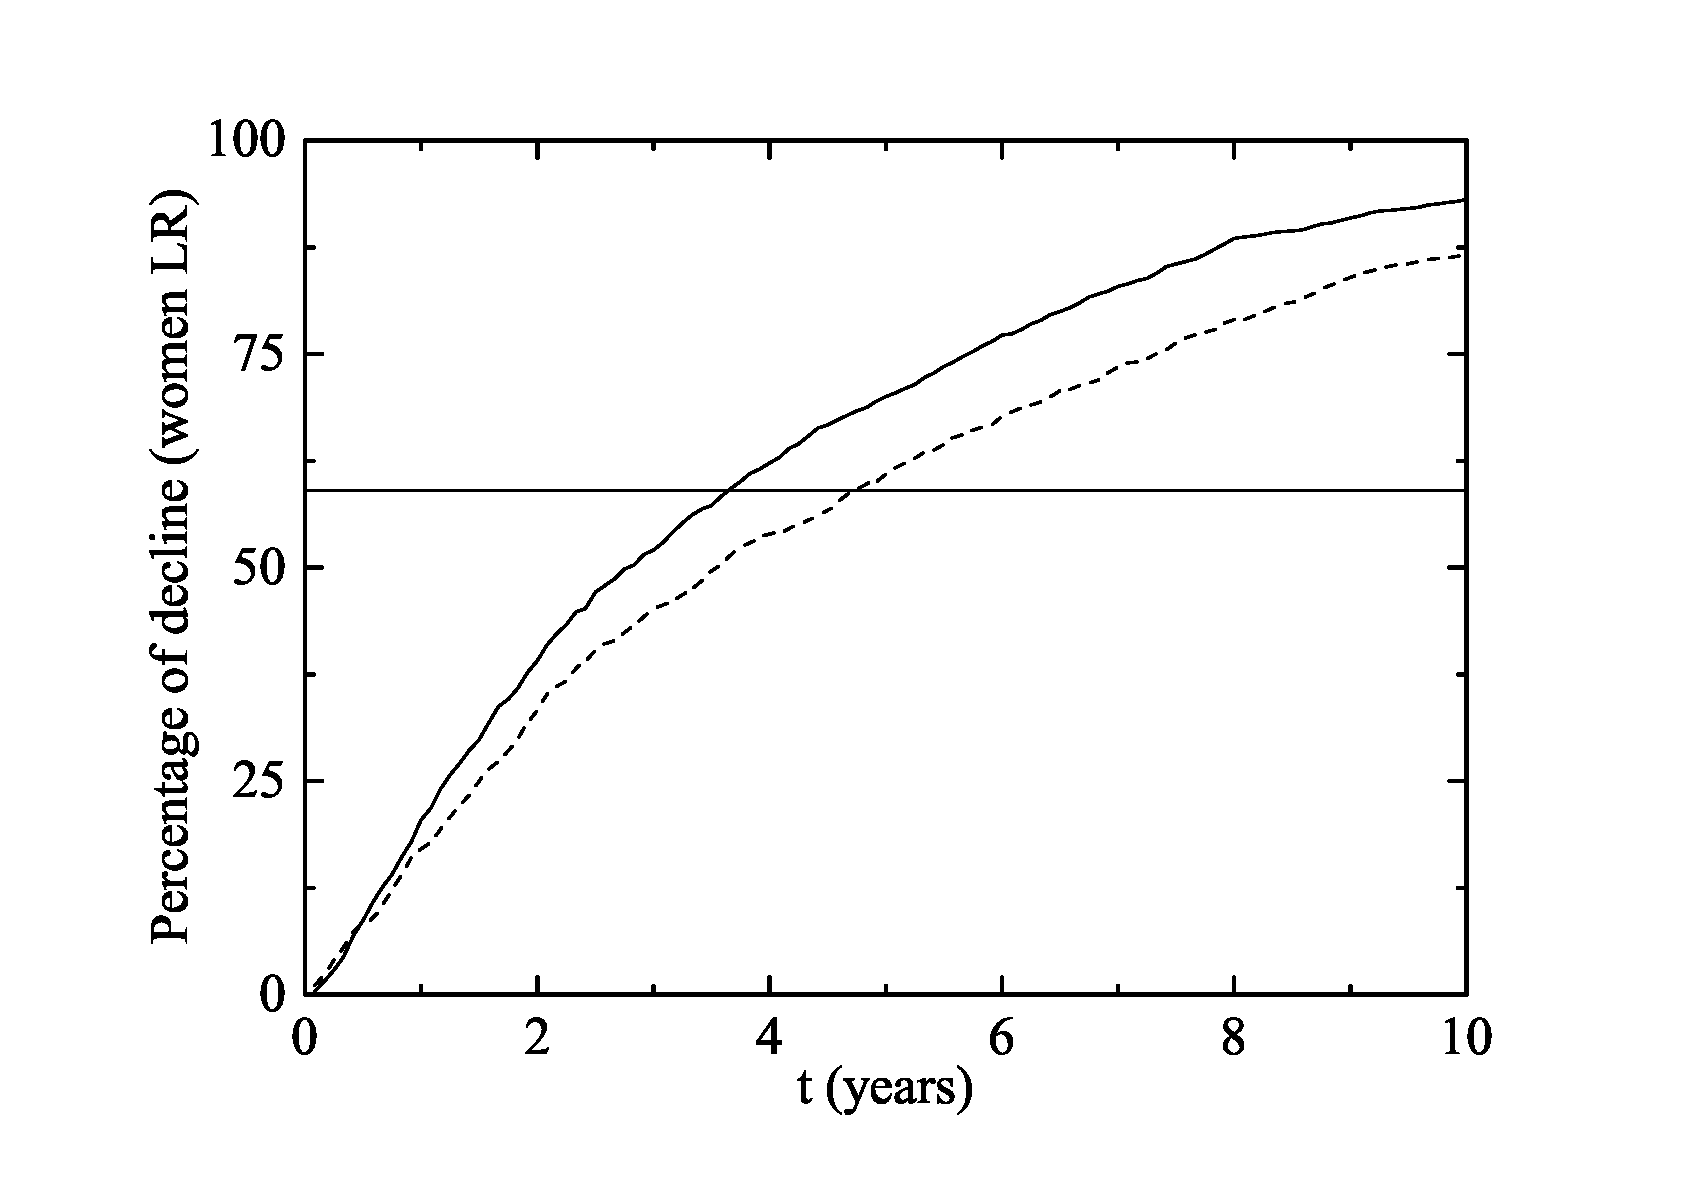
\includegraphics[scale=0.4]{DeclinewomenLR.pdf}
	\vspace{-12pt}
	\caption{Percentage of decline of women aged 14--26 infected of LR HPV 6 and/or 11 (and consequently of GW) after the implementation of the vaccination program in both scenarios (Scenario 1: solid line and Scenario 2: dotted line). The horizontal line represents the percentage of decline in Australian women wart cases after two years.}
	%Pls define. 
	%ANSWER: it is defined in the Introduction, 1st paragraph and GW appears several times along the text. Also, it appears in the list of the abbreviations.
	\label{fig2}
\end{figure}

In our model simulation, after two years of the beginning of the vaccination program, a decline of 33.3--39.1$\%$ has occurred in women and 3.6--4.6 years were necessary to reach the Australian $59\%$ decline rate in GW.

In men aged 14--26 (Figure \ref{fig3}), there was a decline of 23.1--30.5$\%$ after two years and 3--3.75 years were necessary to reach the Australian $39\%$ decline rate of infection. No significant impact on the rate of infection was observed in women or men aged 27--64 in the first $10$ years after the implementation of the vaccination program (Figure \ref{fig4}). It can be explained by the fact that, usually, individuals have sexual intercourses with people more or less the same age.

The herd immunity effect in both scenarios is shown in Figure \ref{fig5} for heterosexual men and  Figure~\ref{fig7} for MSM.  Notice that, in men and MSM, any decline is due to herd immunity. The decline of GW in the whole female population is given in Figure \ref{fig6}. This is predicted when the lines representing their decline are over the vaccination line also shown in this figure. We see that the herd immunity effect starts after $2.58$--$2.91$ years when 11.2--14.45$\%$ of women are vaccinated.
%Figure 8 can not appear before Figure 7. Please check. 
%ANSWER: it has been changed to the right place.

Notice that the herd immunity effect is very clear within the $90\%$ CI both for heterosexual men and women, but it is uncertain in the MSM population. In the best case scenario, the MSM subpopulation achieves a large protection level, but there are other situations in which it remains largely unprotected and the HPV strains still circulate among them for many years. This could be attributed to the way in which the MSM individuals are connected: with a very large number of LSPs among them and some casual links with women with large LSPs. If these women, acting like hubs in the network, are~vaccinated, we obtain a fast eradication of the disease in the MSM population and this would be the best scenario.

\begin{figure}[H]
	\centering
	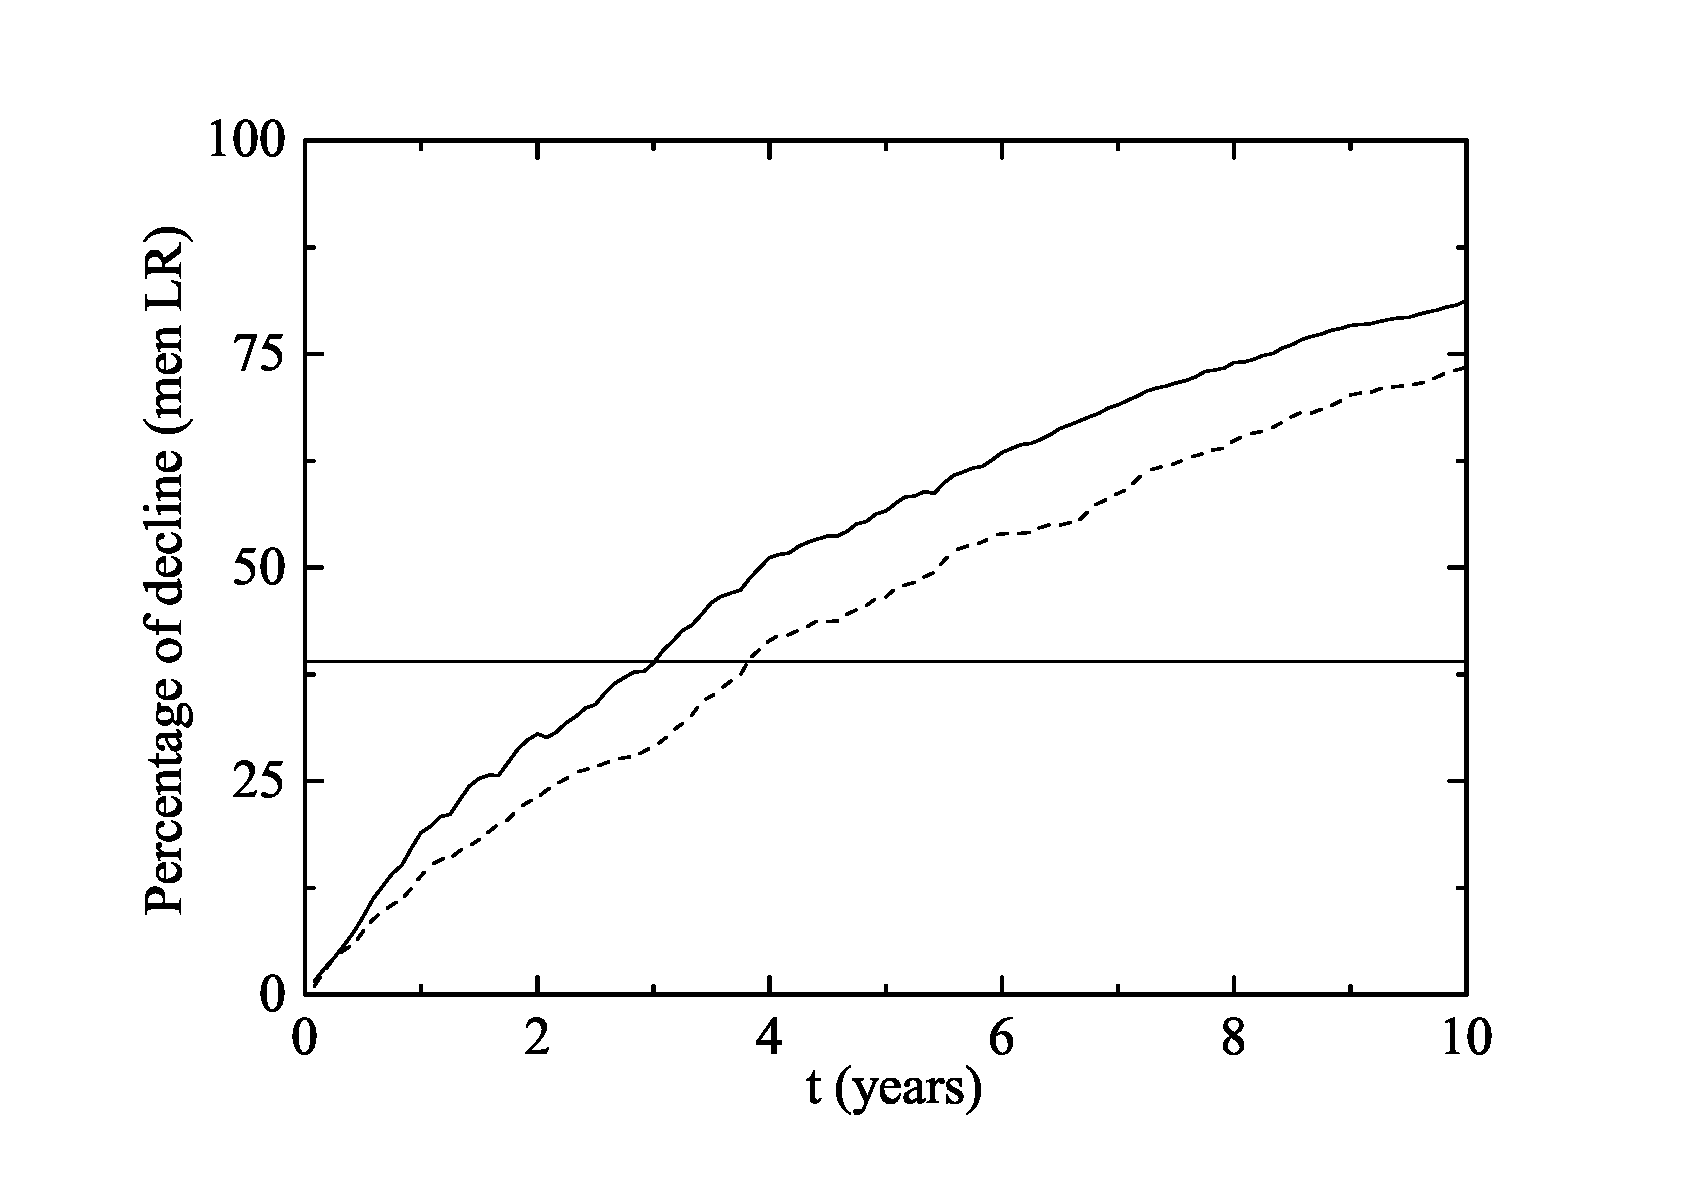
\includegraphics[scale=0.4]{DeclinemenLR.pdf}
	\vspace{-12pt}
	\caption{The same as Figure \protect\ref{fig2} but for men aged 14--26.}
	\label{fig3}
\end{figure}
\vspace{-30pt}

%A simulation of the impact of a program vaccinating 14 years old girls with a coverage of 70\% without catch-up, as for instance, was implemented in Spain, showed that after 2 years the decline in infection in women aged 14-26 with HPV 6 - 11 was about 6\% and 59\% after 8.5 years. On the other hand, the decline in men aged 14-26 infected of HPV 6 - 11 after two years is about 3\% and 39\% after 7.6 years.

%Although this decline refers to infections by HPV 6 and 11 we can expect that it would be very similar for HR HPV genotypes.
\begin{figure}[H]
	\centering
	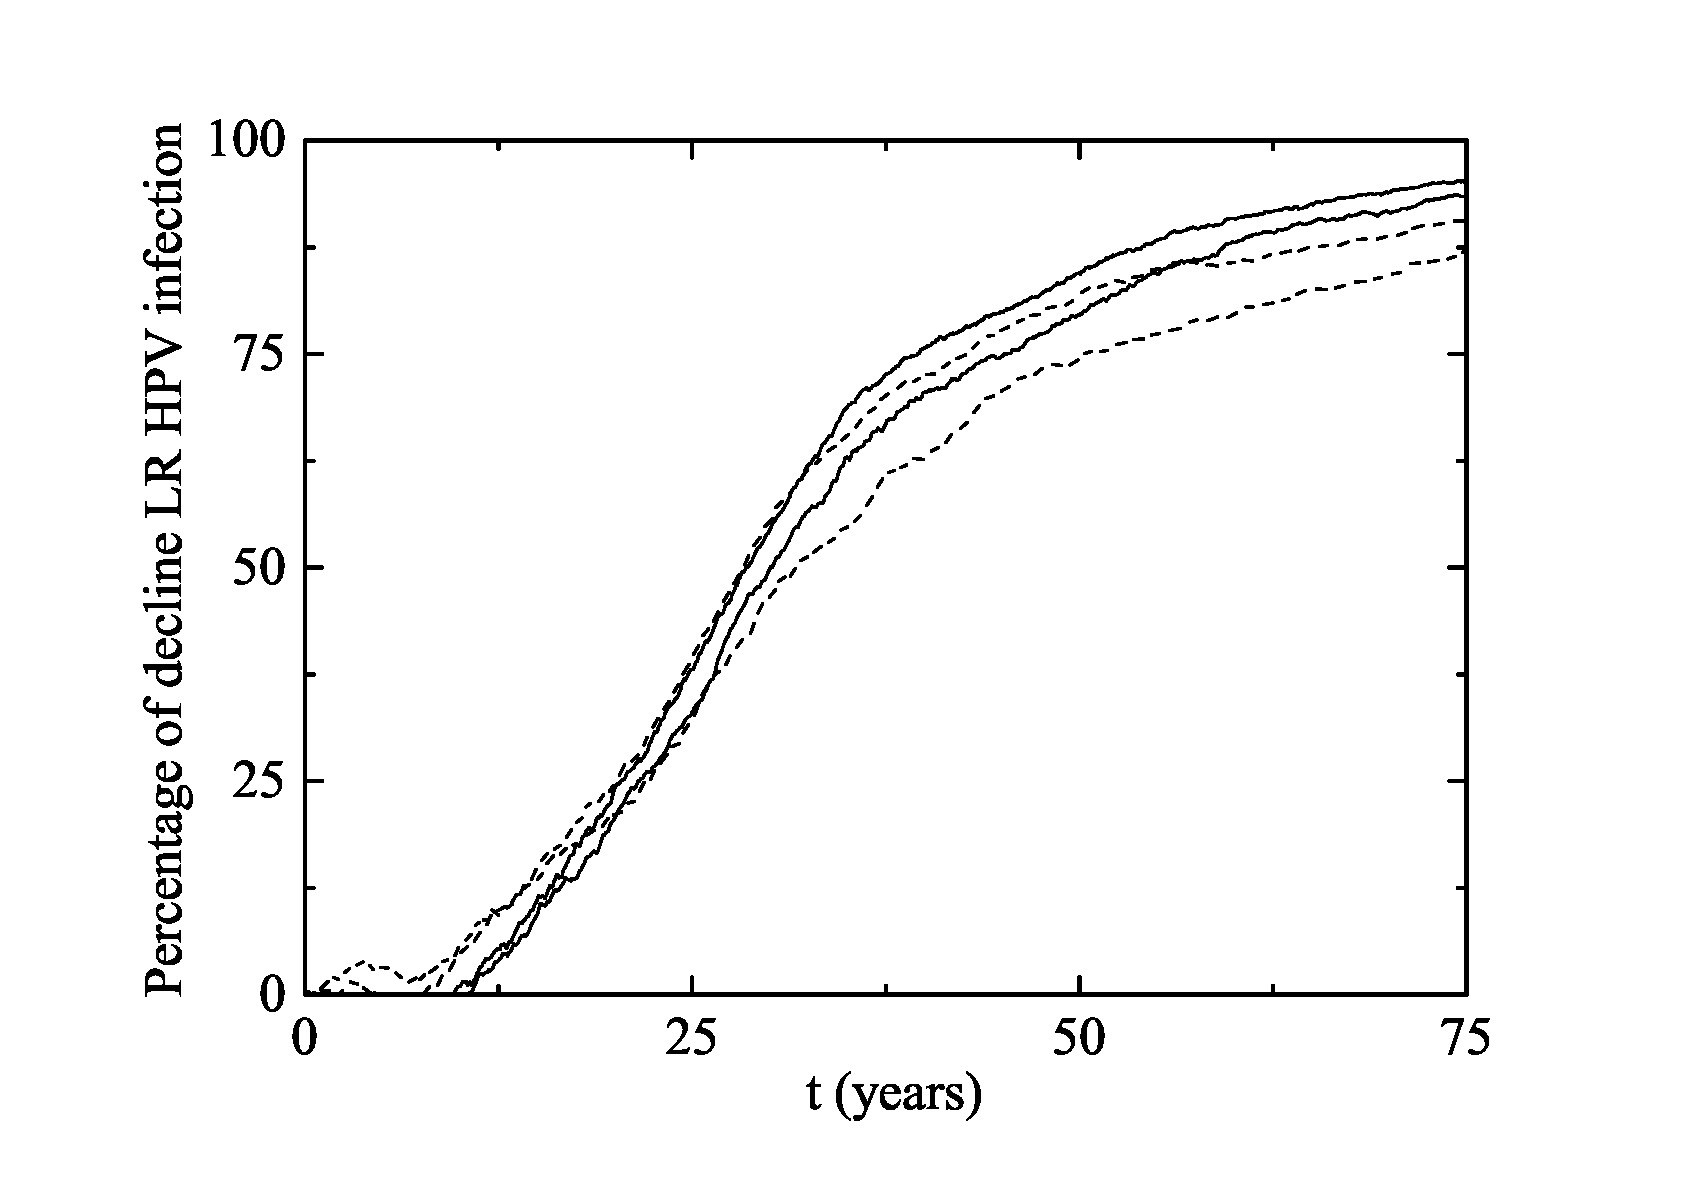
\includegraphics[scale=0.4]{PercentageDeclineolder.pdf}
	\vspace{-12pt}
	\caption{Percentage of decline of men and women aged 27--64 infected of LR HPV 6 and/or 11 (and~consequently of GW) after the implementation of the vaccination program in both scenarios. The~upper solid line corresponds to women in Scenario 1 and the lower solid line corresponds to women in Scenario 2. The upper and lower dotted lines correspond to men in Scenarios 1 and 2, respectively. Notice that no significant decline is observed in women or men aged 27--64 in almost the first 10 years.}
	\label{fig4}
\end{figure}
\vspace{-40pt}

\begin{figure}[H]
	\centering
	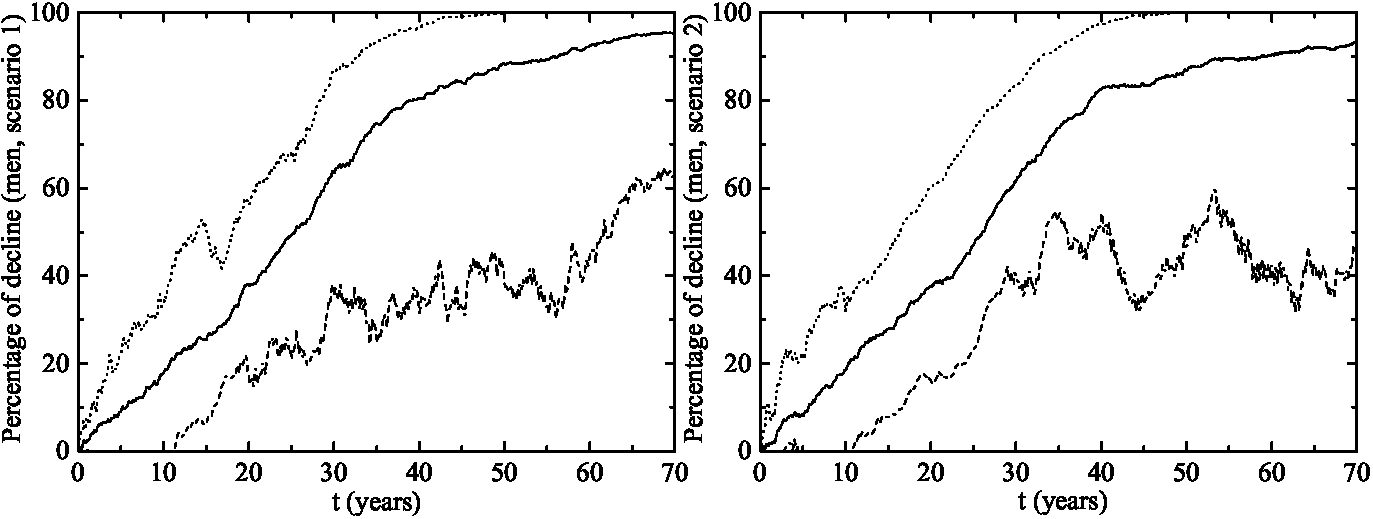
\includegraphics[scale=0.55]{FigHerdImmunity1.pdf}
	\caption{Herd immunity effect of the vaccination program in Australia on heterosexual men (left figure (Scenario 1) and right figure (Scenario 2)). The upper dotted and the lower dashed lines correspond to an interval of 90\% confidence. The solid line
	is the average evolution of the decline in GW.}
	\label{fig5}
\end{figure}
\vspace{-12pt}
\begin{figure}[H]
	\centering
	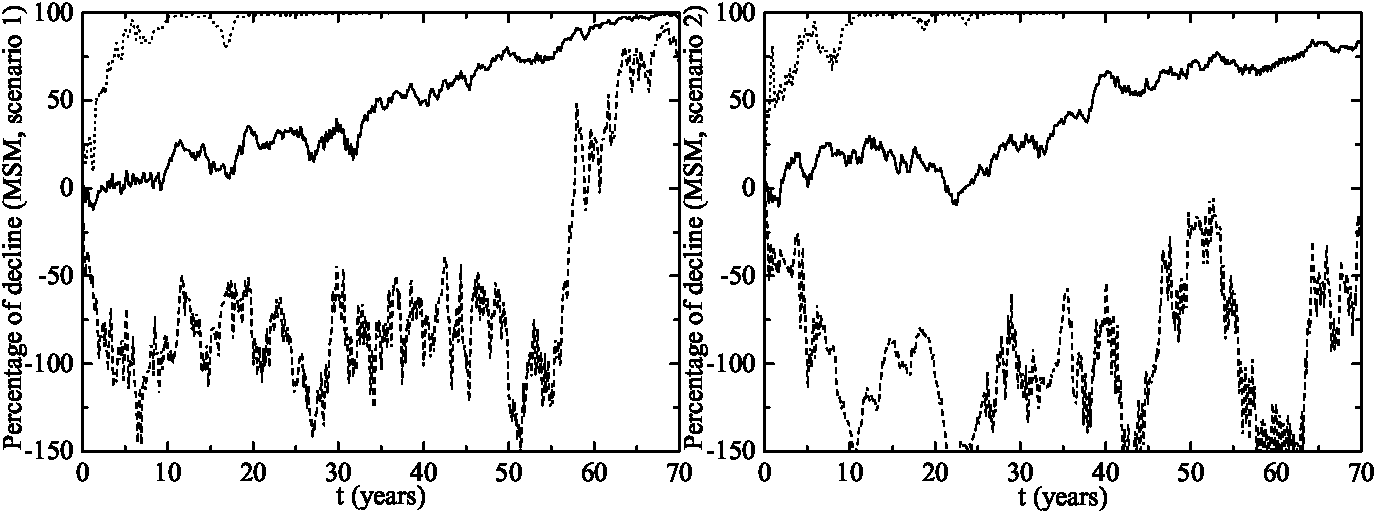
\includegraphics[scale=0.55]{FigHerdImmunity3.pdf}
	\caption{The same as Figure \protect\ref{fig5} but for MSM.}
	%Pls define
	%ANSWER: MSM has been defined in the last paragraph of the Introdiction. It is used several times along the text. Also, it appears in the list of the abbreviations.
	\label{fig7}
\end{figure}
\vspace{-12pt}
\begin{figure}[H]
	\centering
	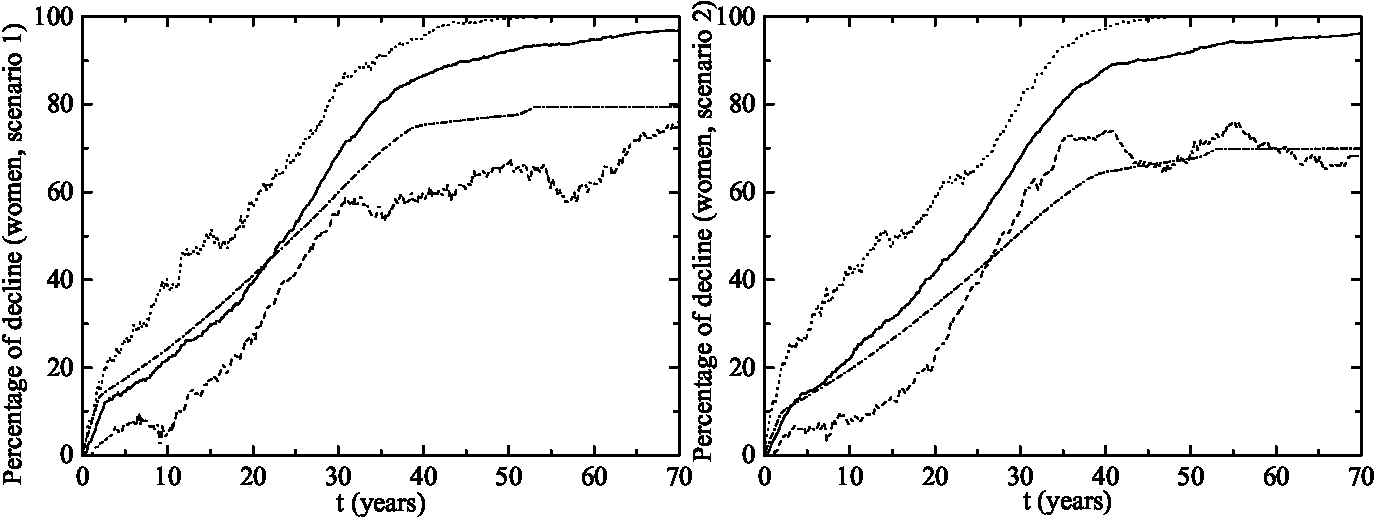
\includegraphics[scale=0.55]{FigHerdImmunity2.pdf}
	\caption{Percentage of decline in GW cases for women for the vaccination program in Australia (left figure (Scenario 1) and right figure (Scenario 2)). The upper dotted and the lower dashed lines correspond to an interval of 90\% confidence. The solid line
	is the average evolution of the decline in GW for the whole female population and the dashed-dotted line is percentage of vaccinated women. Notice~the herd immunity effect also contributes to the decline in the number of infections for unvaccinated women. This can be seen when the decline lines are over the vaccination line.}
	\label{fig6}
\end{figure}